\section{Introduction}
In Astronomy, instruments with higher angular resolution allows us to measure ever smaller structures in the sky. For Radio frequencies, the angular resolution is bound to the antenna dish diameter, which puts practical and financial limitations on the highest possible angular resolution. Radio Interferometers get around this limitation by using several smaller antennas instead. Together, they act as a single large antenna with higher angular resolution at lower financial costs compared to single dish instruments.

SKA
New Radio Interferometers are built
Higher sensitivity
Create images at a hIgher angular resolution
Like MeerKAT
Does not measure the sky image

Difficulty creating an image

And interferometers do not measure the sky directly. Interferometers do not measure the sky in pixels. Each antenna pair measures a Fourier Component. 
But the image reconstruction forms an ill-posed inverse problem
We have many possible images that fit the measurements.
Image reconstruction has to find the most likely image.

But produce a huge amount of data.
larger problem size require distributed computing
so far, it was difficult to separate the image reconstruction
Too much work was multiplied by the number of nodes.
Mostly done on a limited number of shared-memory systems

Target to distribute the image reconstruction
First tests


\subsection{Radio Interferometry System}\label{intro:sys}
This project is focused on distributing Image Reconstruction for Radio Interferometers, which is only one of three steps in the pipeline from measurements to the final image. We give a quick overview over the whole pipeline in figure \ref{intro:system} and how Radio Interferometers work in principle: The antennas observe the arriving electromagnetic wave, gets processed in three steps, Correlation, Calibration and Image Reconstruction. 

\begin{figure}[h]
	\centering
	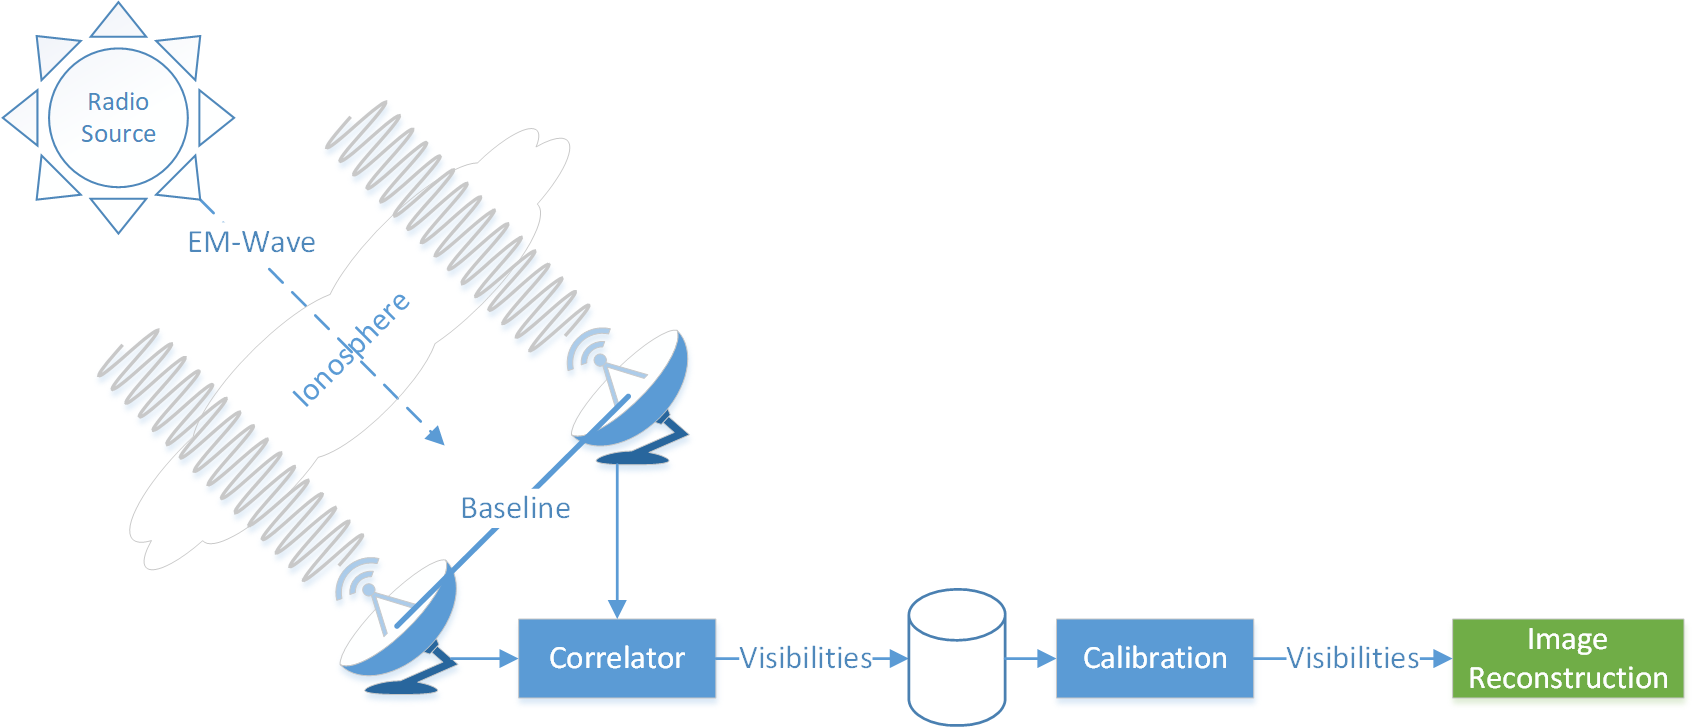
\includegraphics[width=0.80\linewidth]{./chapters/01.intro/system.png}
	\caption{Radio Interferometer System}
	\label{intro:system}
\end{figure}

First, the electromagnetic wave gets measured by the different antennas of the interferometer. The measurements of each antenna pair get correlated into a complex-valued Fourier Component (called Visibility in Radio Astronomy). Each antenna pair measures a noisy amplitude and phase of a single Visibility (Fourier Component) of the sky image. The distance and orientation of the antenna pair relative to the incoming signal, called the baseline, dictates which Visibility gets measured. The longer the baseline the higher-order Visibility gets measured, resulting in a higher angular resolution. After correlation, the Visibility data is saved for later processing.

The Calibration step is done after all Visibility data has been recorded. This step corrects the amplitude and phase of the measurements for varying antenna sensitivities, pointing errors and other effects. Also, this step removes corrupted data from the measurements. After the Visibilities are calibrated, we can average the measurements and reduce the data volume by several factors. Typically, averaging is done to reduce the runtime costs of the Image Reconstruction step.

The Image Reconstruction step takes the calibrated, and potentially averaged down Visibility data and finds the most likely observed image of the sky. Although the Interferometer produces a potentially large number of Visibilities, they are incomplete: For example an Interferometer with dish-antennas is typically blind to the microwave background radiation. The largest structures in the image it can detect depends on the shortest baseline. Since the antennas have to be at least the dish-diameter placed apart, the Interferometer is simply blind to very large structures in the sky image, like the microwave background radiation. This property makes Image Reconstruction Problem ill-posed. In the Image Reconstruction step, we therefore have to find the most likely image which fits the measurements.

\subsubsection{Earth's rotation and arbitrary large Number of Visibilities}
To improve the final image, we want to measure as many different Visibilities as possible. Modern Radio Interferometers use the the earth's rotation to change the baselines. When the earth rotates, it modifies the length of the baseline and by extent, what Visibilities get measured. Modern Interferometer can produce an almost arbitrary large number of measurements by just increasing the observation time.

The data volume can be averaged down in the Calibration step. However, with self-calibration, the Image Reconstruction is tasked with solving both the most likely image and the calibration parameters at the same time. This further improves the reconstruction quality\cite{Wiauxselfcal}, but requires the Image Reconstruction step to handle all the Visibility data.

Modern Radio Interferometers can produce an almost arbitrary large number of measurements. The reconstruction quality benefits from a large number of different Visibility measurements. The two main limiting factors however, are the cost of data storage and the scalability of the Image Reconstruction algorithm.


\subsection{The Image Reconstruction Problem}
For Radio Interferometers, Image Reconstruction forms an ill-posed inverse problem. There are potentially many different images that fit the measurements. The Image Reconstruction is tasked with finding the most likely image $I()$ given the (calibrated) Visibility measurements $V()$. Formally, we want to invert the measurement equation of the Radio Interferometer. Equation \eqref{intro:inverseproblem} shows a measurement equation for Radio Interferometers, and figure \ref{intro:inversefig} shows an example for $V()$ and $I()$.

\begin{figure}[htp]
	% preliminary
	\sbox\twosubbox{%
		\resizebox{\dimexpr.9\textwidth-1em}{!}{%
			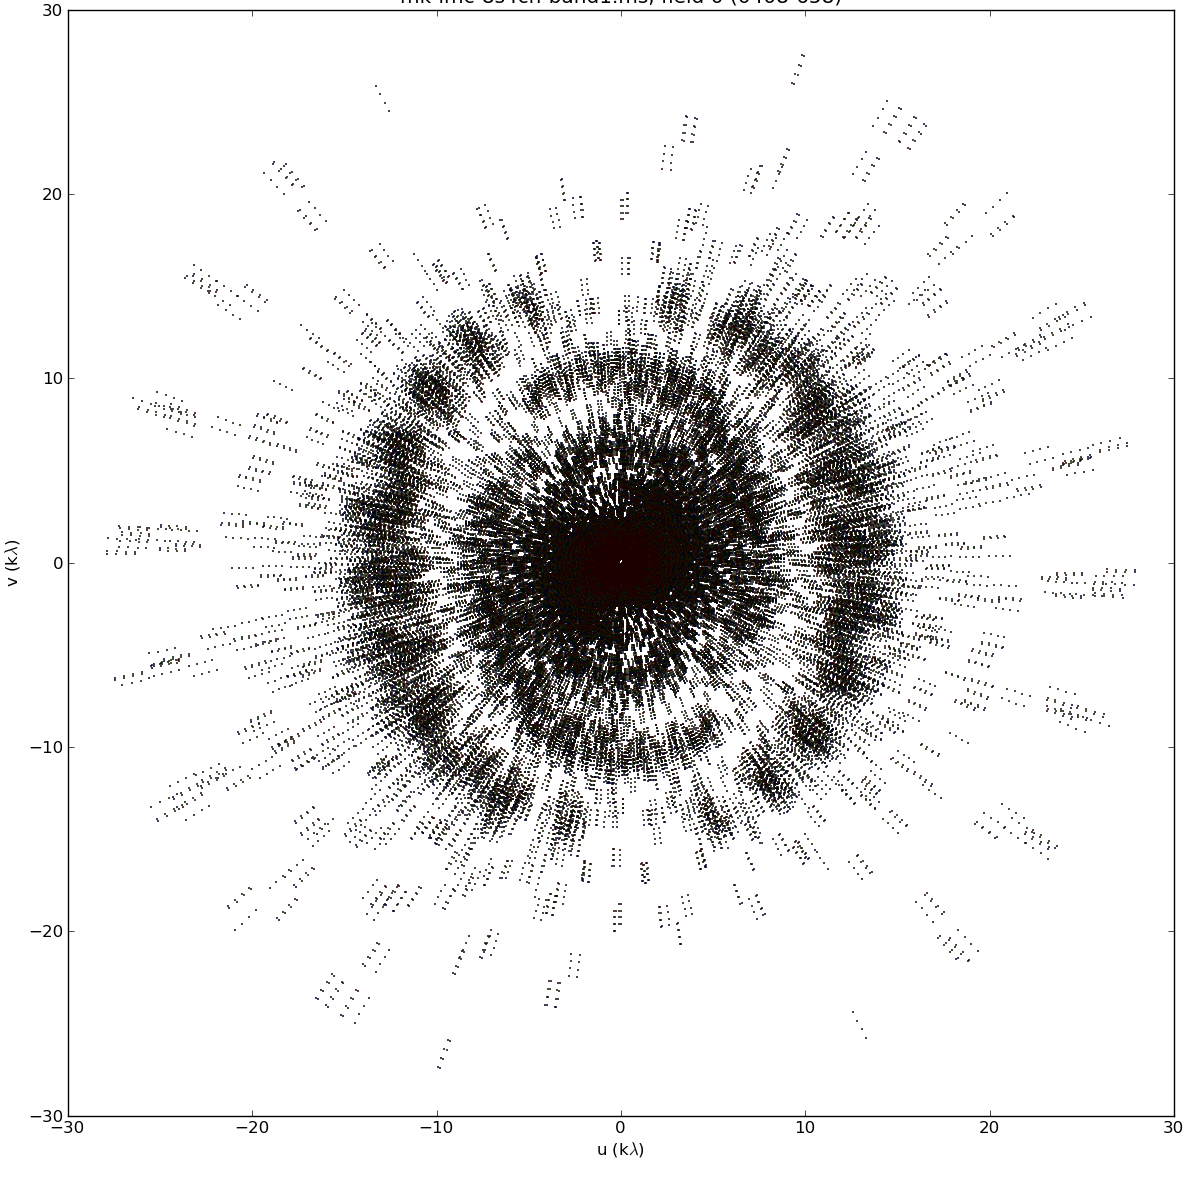
\includegraphics[height=3cm]{./chapters/01.intro/meerkat_uv2.png}%
			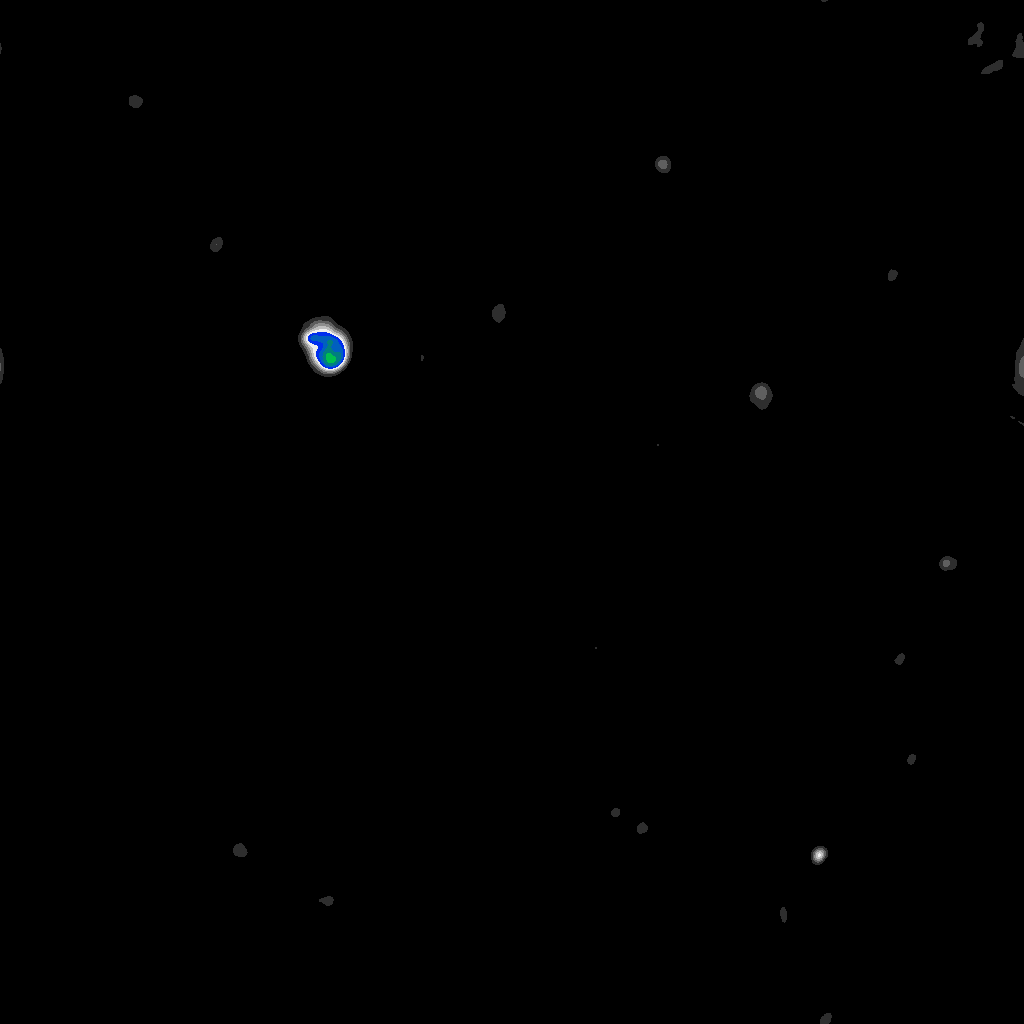
\includegraphics[height=3cm]{./chapters/01.intro/mk2/clean.png}%
		}%
	}
	\setlength{\twosubht}{\ht\twosubbox}
	
	% typeset
	\centering
	\subcaptionbox{Measurements $V()$ in the UV plane.\label{intro:inversefig:uvspace}}{%
		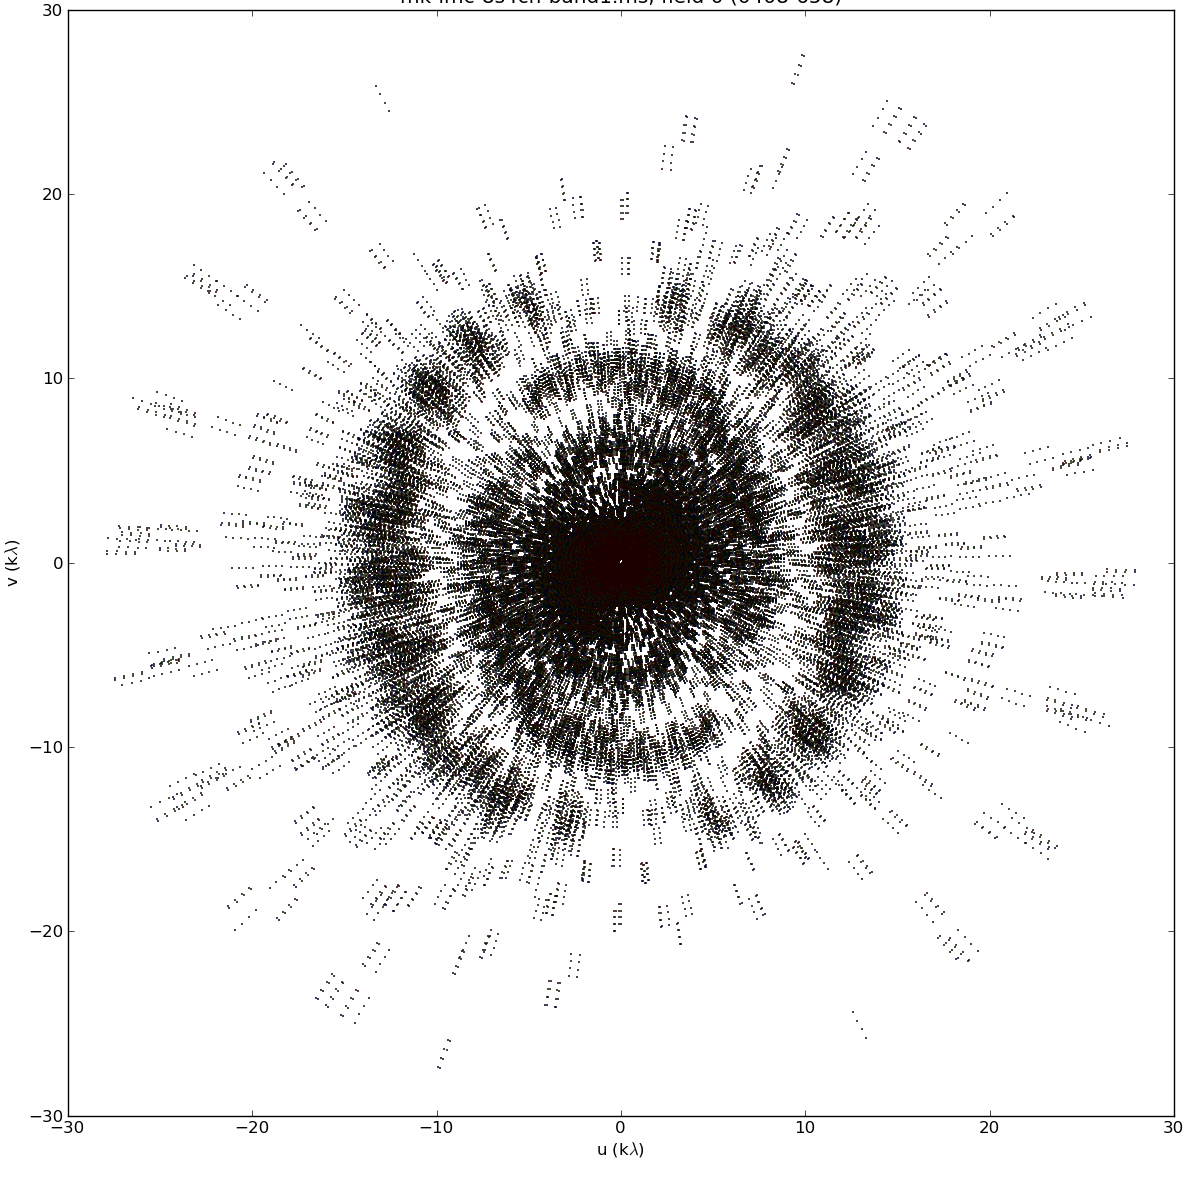
\includegraphics[height=\twosubht]{./chapters/01.intro/meerkat_uv2.png}%
	}\quad
	\subcaptionbox{The observed image $I()$.\label{intro:inversefig:reconstruction}}{%
		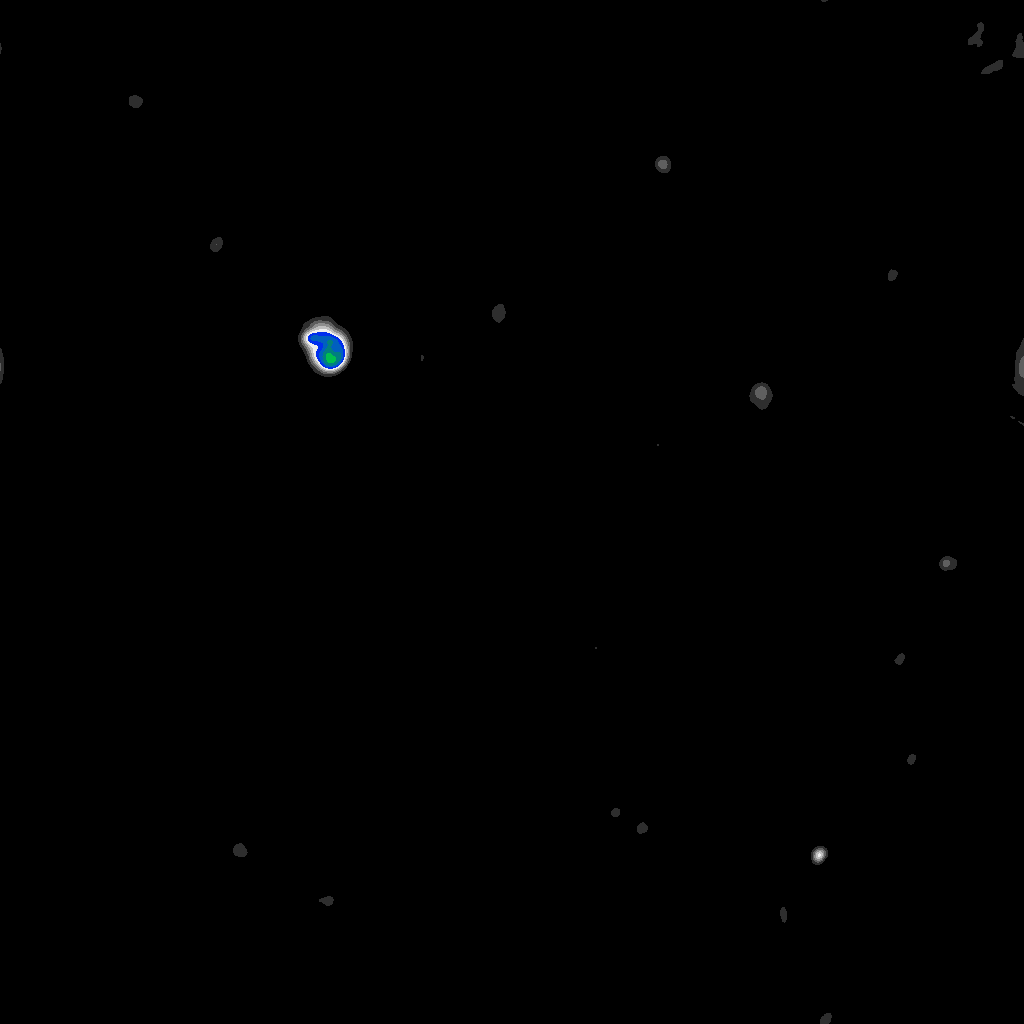
\includegraphics[height=\twosubht]{./chapters/01.intro/mk2/clean.png}%
	}
	\caption{The Image Reconstruction Problem}\label{intro:inversefig}
\end{figure}

\begin{equation}\label{intro:inverseproblem}
V(u, v, w) = \int\int  \frac{I(x, y)}{c(x, y)}  e^{2 \pi i [ux+vy+ w(c(x, y) - 1)]} \: dx \: dy \quad \quad c(x,y) = \sqrt{1 - x^2 - y ^2}
\end{equation}

The measurement equation \eqref{intro:inverseproblem} contains three parts. The Visibility measurements $V(u,v,w)$, the observed image with a normalization factor $\frac{I(x, y)}{c(x, y)}$ and the Fourier Transform $e^{2 \pi i (\ldots)}$. The $x$ and $y$ coordinates are angles from the image center. A pixel in $I(x,y)$ represents how strong the radio emission is from the direction. Note that the Visibilities $V(u,v,w)$ are three dimensional, while the image $I(x,y)$ only has two. However, also note that the third component $w$ only depends on the directions $x$ and $y$. In a sense, the Visibilities $V()$ and the Image $I()$ have a two dimensional Fourier relationship, but with a directionally dependent correction $e^{2 \pi i (\ldots +w(c(x, y) - 1))}$. 

The third component $w$ is an example of a Directionally Dependent Effect (DDE) which have a tendency to increase the runtime costs of the Image Reconstruction. The $w$-component keeps us from using the Fast Fourier Transform (FFT) for the measurement equation \eqref{intro:inverseproblem}. Research in this area tries to use approximations which lets us use faster algorithms like the FFT, and correct for DDE's accurately enough \cite{veenboer2017image, offringa2014wsclean, pratley2018fast}. In this project, the $w$-correction is the only DDE we handle.

\subsubsection{System of Linear Equations}\label{intro:linear}
Even though the Fourier Transform in equation \eqref{intro:inverseproblem} contains a $w$-correction factor, $V()$ and $I()$ have still a linear relationship. This means we can represent the Image Reconstruction Problem as a system of linear equations: \eqref{intro:linear:linear}. $F$ is the Fourier Transform with $w$-correction, $x$ is the image we are searching and $V$ are the measured Visibilities\footnote{$V$ in the equation \eqref{intro:linear:linear} is a vector. We use the lower-case $v$ to denote the axis in the Fourier space $uvw$, while the upper-case letter denotes the Visibility-vector.}

\begin{equation}\label{intro:linear:linear}
\underset{x}{find}\quad V = Fx
\end{equation}

Incompleteness \ref{intro:inversefig:uvspace}. The further we move away from the center, the lower the sample density. (Hole in the center, but not visibile due to resoultion limitations). Non-uniform sampling pattern in the UV-space. Sampling pattern defined by the instrument layout
As we discussed in section \ref{intro:sys}, Radio Interferometers can produce an almost arbitrary large number of Visibilities.
Overdetermined system. More Visibilities $V$ than pixels in the image $x$.
But noisy. So we cannot find a solution to  \eqref{intro:linear:linear}. We need to account for noise, so we arrive at a similar equation \eqref{intro:linear:l2}

\begin{equation}\label{intro:linear:l2}
\underset{x}{find} \: \left \| V - Fx \right \|_2^2 < \epsilon
\end{equation}

We want to find a solution $x$ which below the noise level
This is a convex optimization problem.
Not a unique solution. Potentially many $x$ which satisfy \eqref{intro:linear:l2} (because of the incompleteness).
We cannot find the true $x$ from the Visibility measurements alone. 
Which makes the whole inverse problem ill-posed.
However, in practice we can do something else. We can use prior information about the image and rank the candidates for \eqref{intro:linear:l2} from most likely to unlikely.
When we look at \ref{intro:inversefig:reconstruction}, we see it has stars, and extended emissions, clouds. 

Theory of Compressed Sensing

$F$ is too big for any practical application. It has the size of pixels times Visibilities. 4k*4k pixels, times 4 billion Visibilities.


\subsubsection{Different Representations for the Image Reconstruction Problem}
$F = M W\: FFT(x)$
Masking Matrix $M$
Different ways of representing the image reconstruction problem.

\begin{alignat}{2}
\text{in-painting:}\: \underset{V_{Unif}}{find}&\quad MV_{Unif} = V,  \quad &I = iFFT(V_{Unif})\\
\text{deconvolution:}\: \underset{I}{find}&\quad I \star PSF = I_{Dirty},  \quad &I_{Dirty} = F^{-1}V
\end{alignat}

Explain in-painting
explain deconvolution

Deconvolution is used
To our knowledge, in-painting is not used for Radio Interferometer image reconstruction.

Decide on a representation!




\subsection{Solving the Image Reconstruction Problem: The Major/Minor Cycle architecture}
Current state of the art way of solving the image reconstruction problem. Major Minor Cycle architecture.
Representation: Deconvolution.
The Major Cycle is a fast approximation of the Transform Matrix $F$.
The Minor Cycle is a deconvolution algorithm. In this architecture, the Deconvolution algorithm is responsible for including prior knowledge about the image.

\begin{figure}[h]
	\centering
	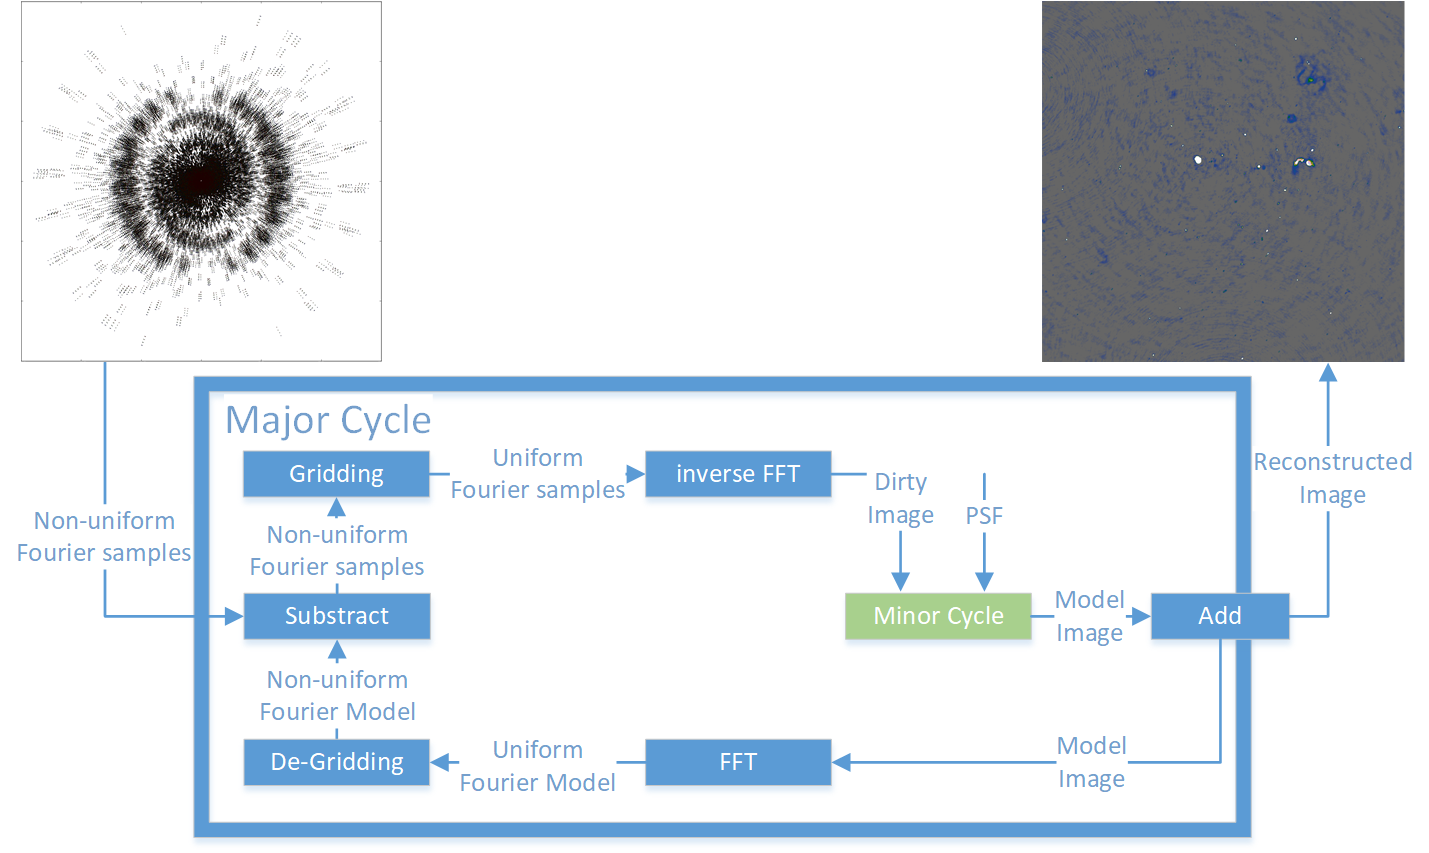
\includegraphics[width=0.80\linewidth]{./chapters/02.hypo/Major-Minor3.png}
	\caption{The Major Cycle Architecture}
	\label{intro:major}
\end{figure}

The Gridder + FFT is responsible for a fast approximation of $F$, while the deconvolution algorithm
Gridder is responsible for handling all Radio Interferometry weirdness. It has to handle the $w$-term of the Visibilities \eqref{intro:inverseproblem}. In practice, even more corrections fall onto the job of the Gridder. Since we have magnitudes more Visibilities than pixels, the Gridder's job is to "compress" the problem.

Note on the Cyclic Nature. It is counter intuitive and explained later in 

\subsubsection{The Gridder}


\subsubsection{Minor Cycle: CLEAN Deconvolutions}
Contains two classes of objects: Point sources, which are essentially stars, and extended emissions, which span over several pixels.


\subsubsection{Why are there Major Cycles in the first place?}
\begin{figure}[h]
	\centering
	\begin{subfigure}[b]{0.3\linewidth}
		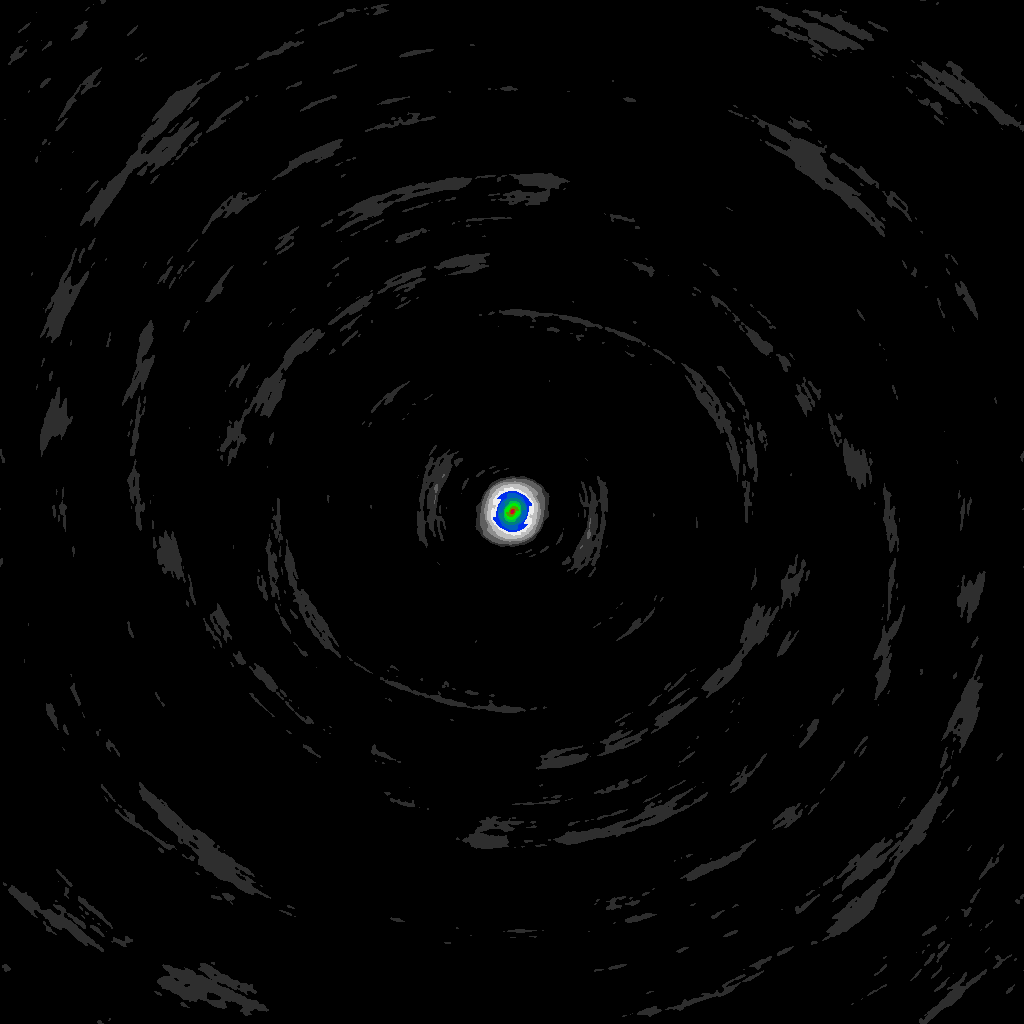
\includegraphics[width=\linewidth]{./chapters/01.intro/mk2/psf.png}
		\caption{Point Spread Function.}
		\label{results:points:tclean}
	\end{subfigure}
	\begin{subfigure}[b]{0.3\linewidth}
		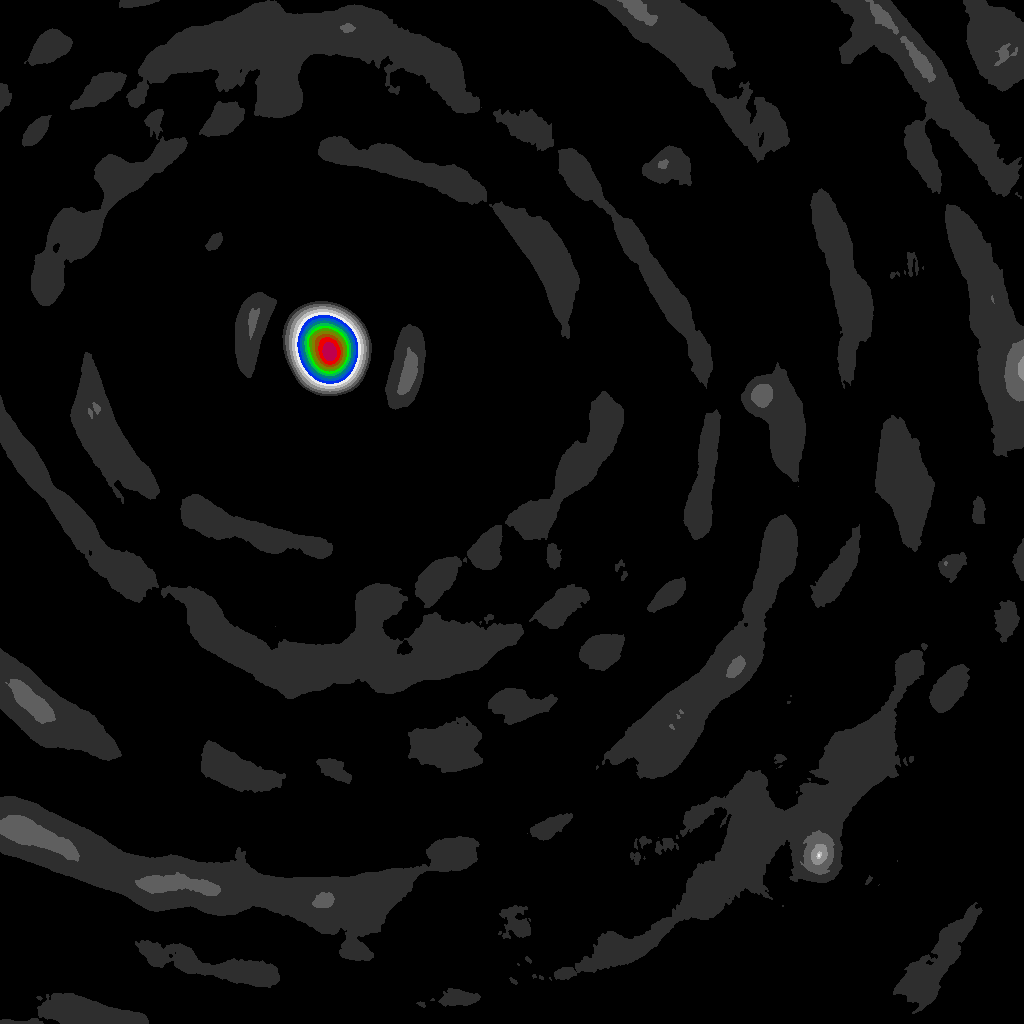
\includegraphics[width=\linewidth]{./chapters/01.intro/mk2/dirty.png}
		\caption{Dirty image}
		\label{results:points:tclean}
	\end{subfigure}
	\begin{subfigure}[b]{0.3\linewidth}
		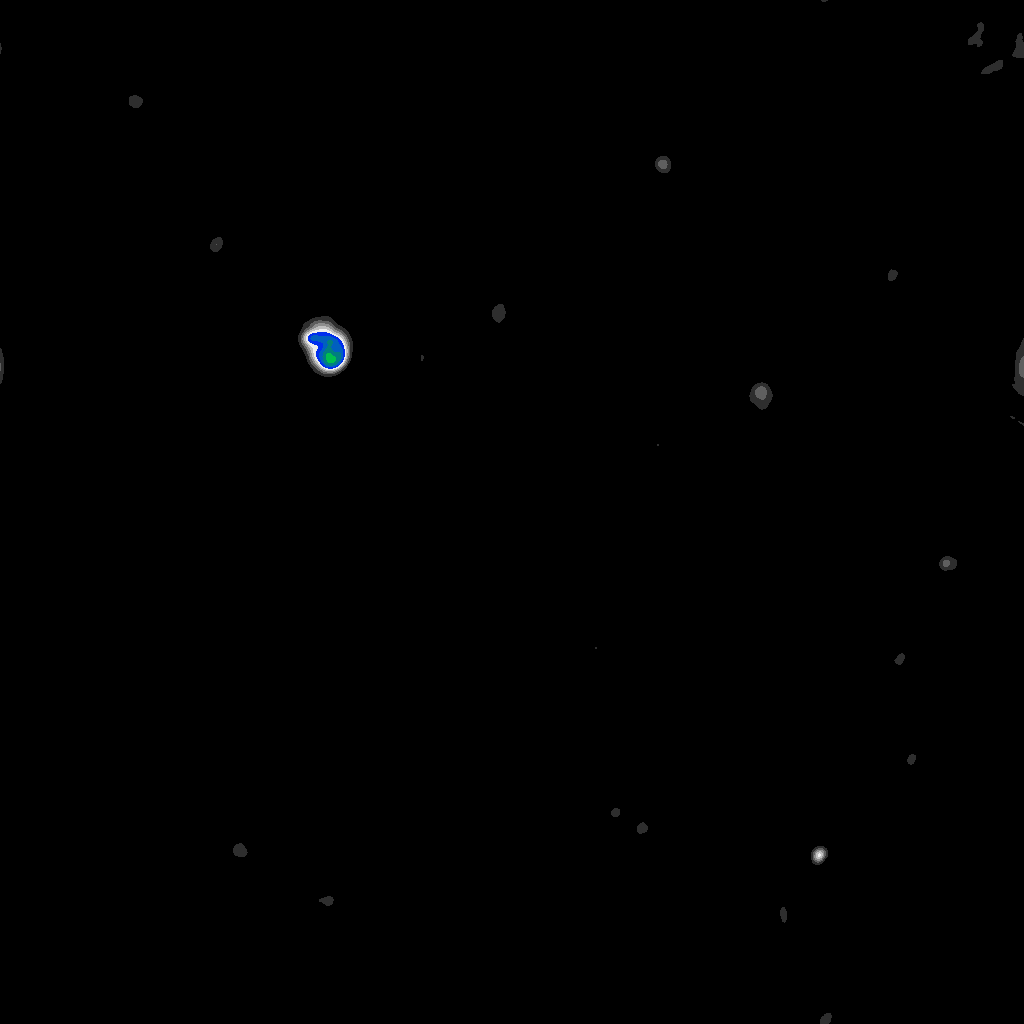
\includegraphics[width=\linewidth]{./chapters/01.intro/mk2/clean.png}
		\caption{Deconvolved image.}
		\label{results:points:tclean}
	\end{subfigure}
	
	
	\caption{Image reconstruction of two simulated point sources.}
	\label{results:points}
\end{figure}
Find the fainter sources in later iterations
Because we can only estimate the psf.



\subsection{Distributing the Major and Minor Cycles}
Difficulty in separation
Each Pixel depends on all Visibilities, and a single Visibility depends on all pixels.
Doing work several times

\subsubsection{Compressed Sensing and the evolution of Priors}
Positivity constraint.
Contains two classes of objects: Point sources, which are essentially stars, and extended emissions, which span over several pixels.


\subsection{The Major Cycle Architecture}
Major cycle how to reconstruct the image with deconvolution
In an efficient manner

$V()$ problems of non-uniform sampling, and the 3 dimensions. keep us from using the Fast Fourier Transform.
We first interpolate on a regularly spaced grid, in the "Gridder".
Use the FFT. For large numbers of Visibilities, this is faster. than inverting equation directly \eqref{intro:inverseproblem}.
And now we do a deconvolution in image space

So we have three basic components, Gridder, FFT and Deconvolution algorithms.
The Major Cycle Architecture makes this a cycle.
Shown in figure \ref{intro:major}.



Why the cycle is necessary



\subsubsection{Minor Cycle}


